\section{Method}

\begin{frame}
\frametitle{Method}
\framesubtitle{Overview}

\begin{figure}
    \centering
    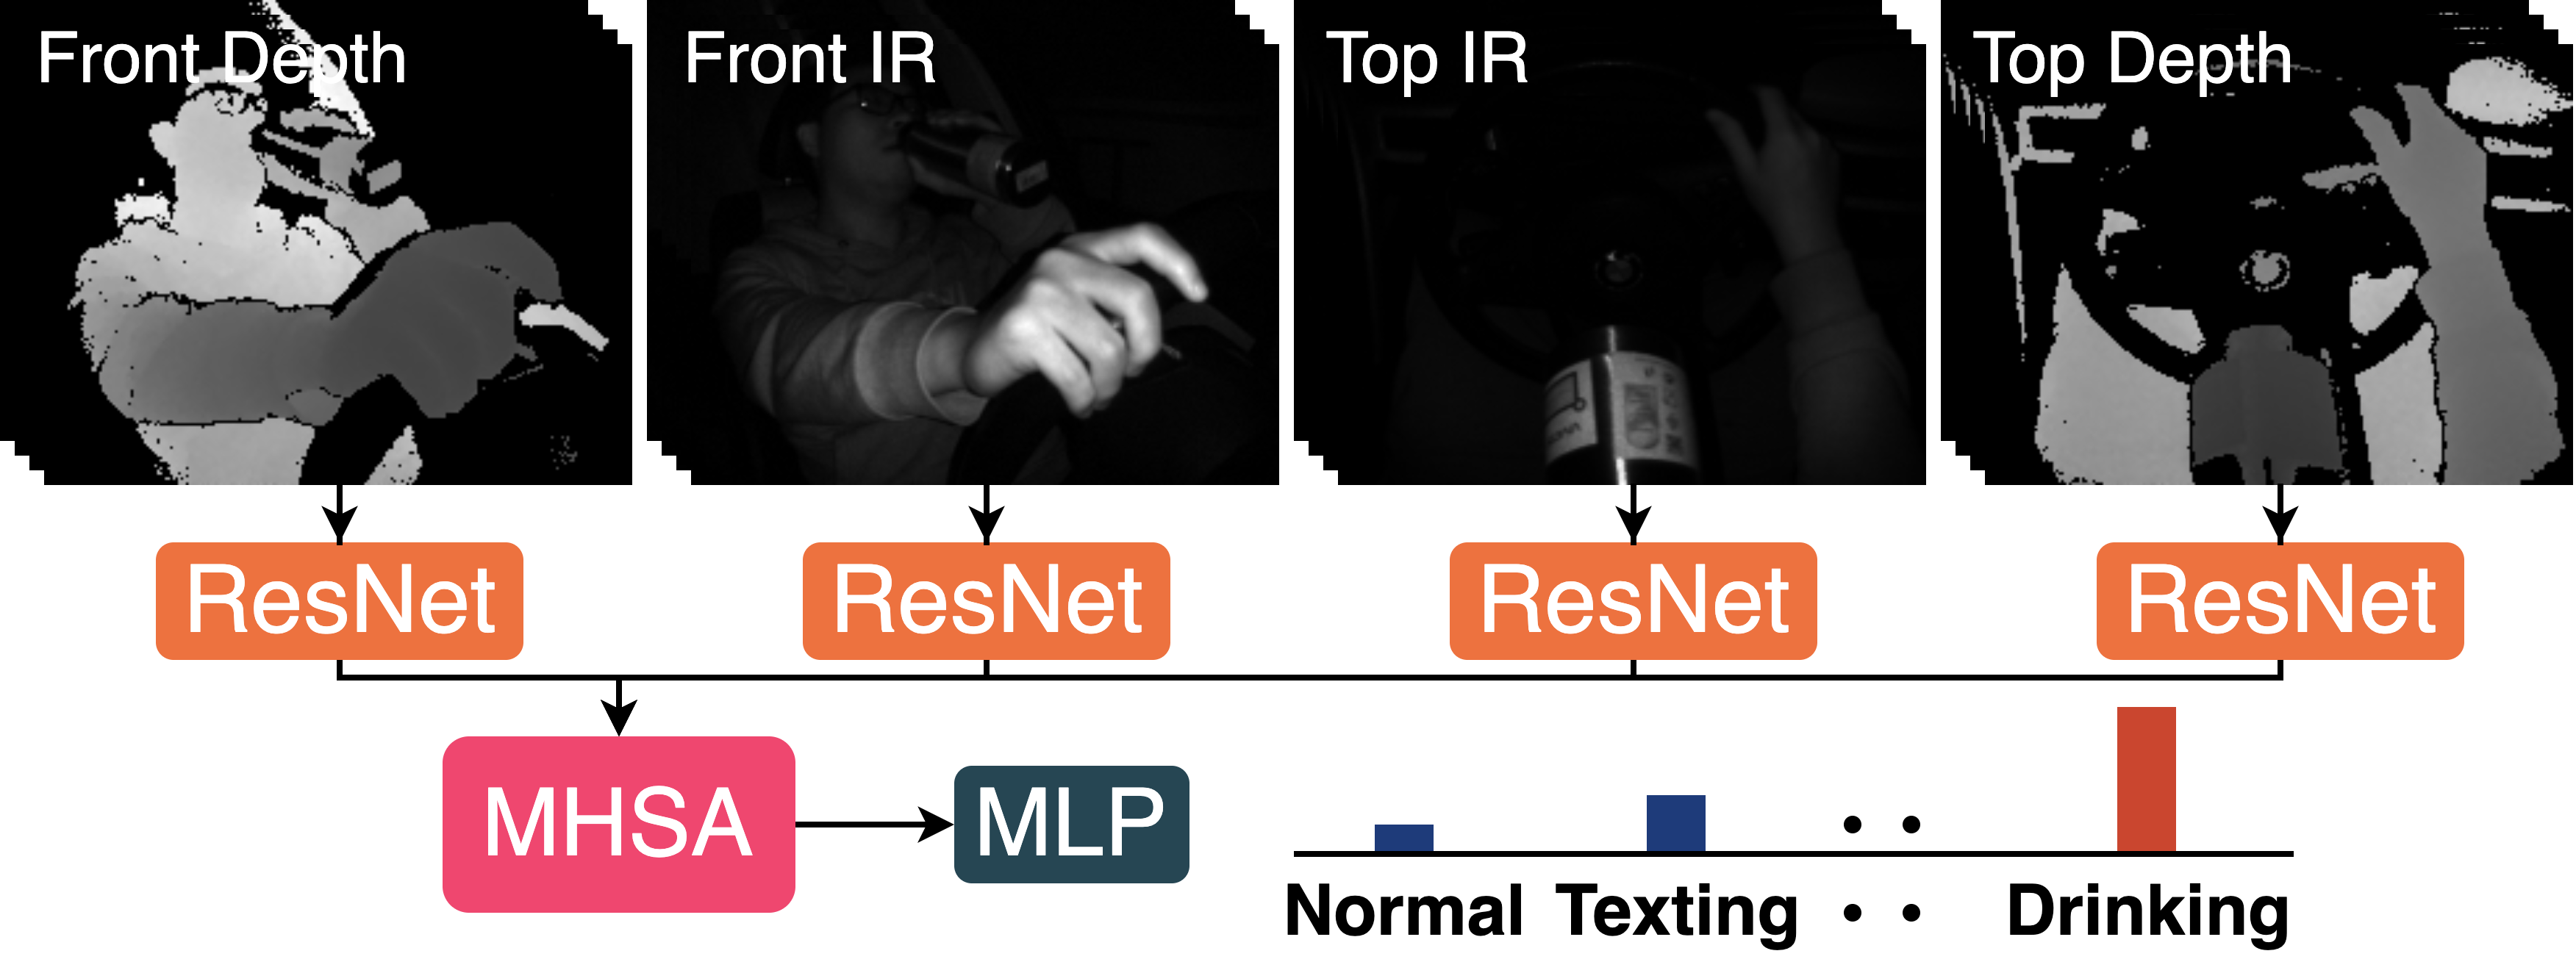
\includegraphics[width=0.9\textwidth]{images/overview.png}
    \caption{An overview of our proposed DMS.}
    \label{fig:4}
\end{figure}
\end{frame}

\begin{frame}
\frametitle{Method}
\framesubtitle{Overview}

\begin{enumerate}
    \item We first use R3D-18 \cite{tran2018closer} to extract spatiotemporal features from the input multiview multimodal videos. 
    \item We the feed the feature maps to our masked multi-head self-attention module to interact and fuse the features.
    \item We also used the supervised contrastive learning based on MoCo \cite{he2020momentum} to facilitate training.
    \item The classifier is co-trained under the supervision of the cross-entropy loss.
\end{enumerate}

\end{frame}

\begin{frame}
\frametitle{Method}
\framesubtitle{Multi-Head Self-Attention Fusion}

\begin{figure}
    \centering
    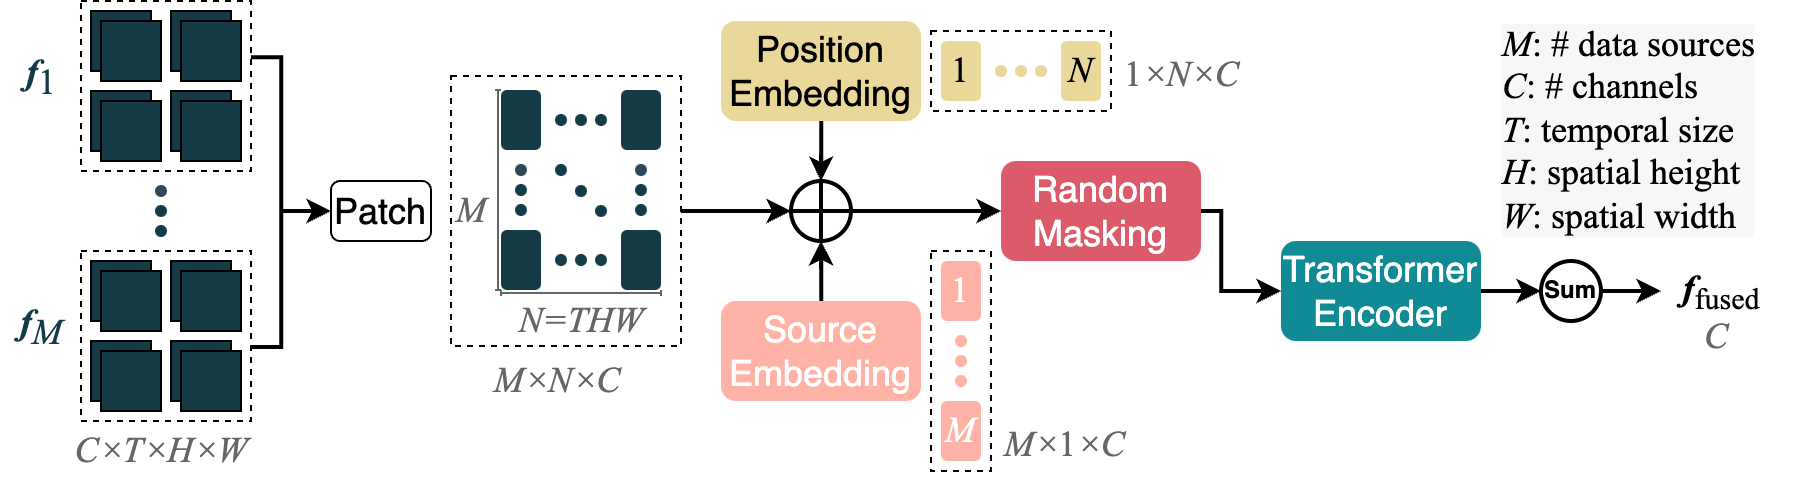
\includegraphics[width=\textwidth]{images/fusion_mhsa_2.png}
    \caption{The architecture of our masked multi-head self-attention module.}
    \label{fig:5}
\end{figure}

\end{frame}

\begin{frame}
\frametitle{Method}
\framesubtitle{Other Fusion Methods}

\begin{figure}
    \centering
    \begin{subfigure}[b]{0.45\textwidth}
        \centering
        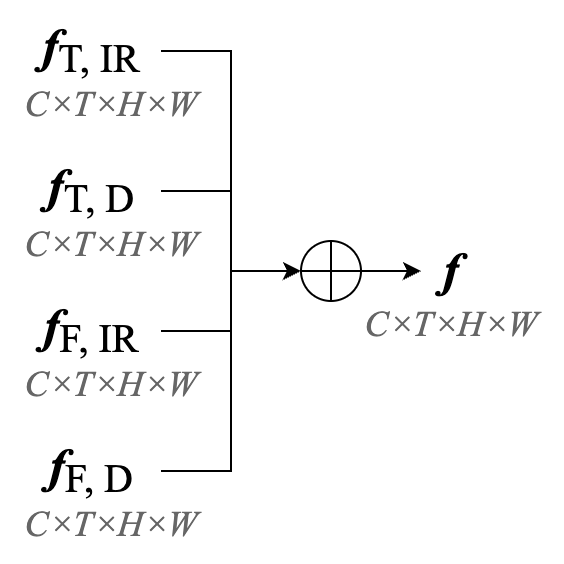
\includegraphics[height=11em]{images/fusion_sum.png}
        \caption{Sum.}
        \label{fig:6.a}
    \end{subfigure}
    \hskip 1em
    \begin{subfigure}[b]{0.45\textwidth}
        \centering
        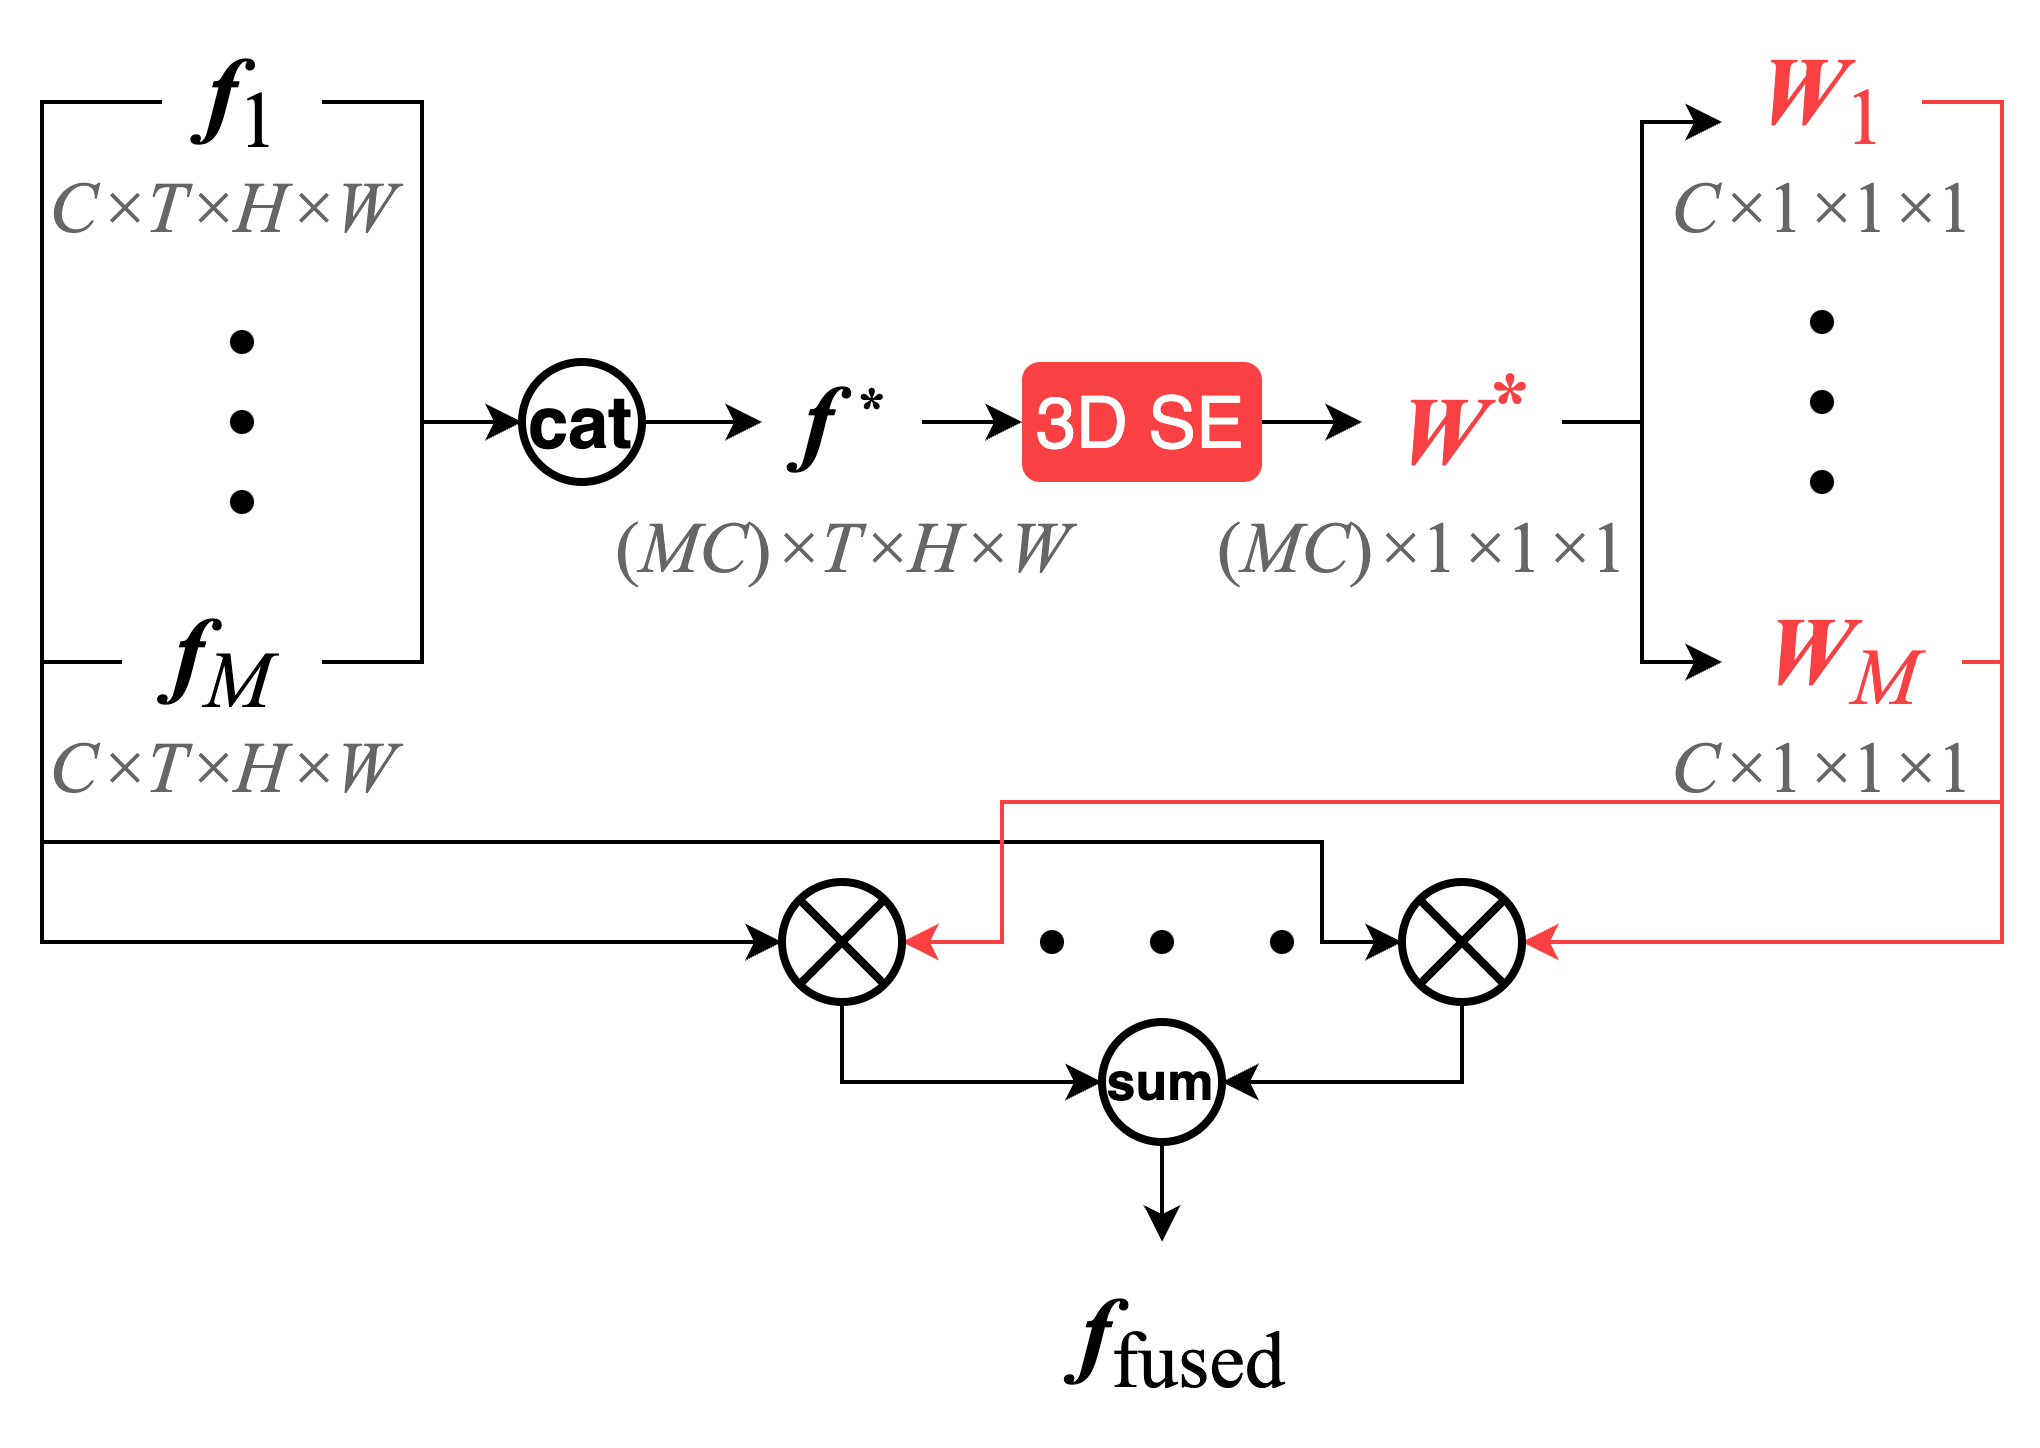
\includegraphics[height=11em]{images/fusion_se.png}
        \caption{SE.}
        \label{fig:6.b}
    \end{subfigure}
    \caption{The architectures of the other fusion methods.}
    \label{fig:6}
\end{figure}

\end{frame}